\documentclass[handout, serif, aspectratio=169, 10pt]{beamer}

% packages
%\usepackage{newpxmath} % math font is Palatino compatible
%\usepackage[nomath]{fontspec}

\usepackage{setspace}
\usepackage{xcolor}
\usepackage{soul} % for \st
\usepackage{hyperref} % for links
\definecolor{links}{HTML}{2A1B81}
\hypersetup{colorlinks,linkcolor=,urlcolor=links}


% table stuff
\usepackage{chronosys}
\usepackage{verbatim}
% \pagenumbering{arabic}
\usepackage{tabularx}
\usepackage{booktabs}
\usepackage{ragged2e}
\usepackage{mathtools}

% R Code
\usepackage{listings}
\usepackage{courier}
\lstset{basicstyle=\scriptsize\ttfamily,breaklines=true}
\lstset{framextopmargin=50pt,frame=bottomline}

% themes
\usetheme[progressbar=frametitle, block=fill]{metropolis}
\useoutertheme{metropolis}
\useinnertheme{metropolis}

% colors
\definecolor{dimwhite}{rgb}{0.99, 0.99, 0.99}
\definecolor{charcoal}{rgb}{0.21, 0.27, 0.31}
\definecolor{slategray}{rgb}{0.44, 0.5, 0.56}
\definecolor{dimgray}{rgb}{0.41, 0.41, 0.41}
\definecolor{bleudefrance}{rgb}{0.19, 0.55, 0.91}

% beamer options
\setbeamercolor{author}{fg=charcoal}
\setbeamercolor{background canvas}{bg=white}
\setbeamercolor{section in toc}{fg=charcoal}
\setbeamercolor{subsection in toc}{fg=dimgray}
\setbeamercolor{frametitle}{bg=dimwhite, fg=charcoal}
\setbeamercolor{progress bar}{fg=slategray, bg=fg!50!black!30}
\setbeamercovered{transparent}
\setbeamertemplate{itemize items}[triangle]
\setbeamertemplate{itemize subitem}[circle]
\setbeamertemplate{itemize subsubitem}[square]
\setbeamersize{text margin left=7mm,text margin right=7mm} 

% new commands
\newcommand{\q}[1]{``#1''}
\newcommand{\hs}[1]{\textsc{\hfill\scriptsize\color{dimgray}#1}}
\newcommand{\g}[1]{{\color{gray}#1}}
\newcommand{\dg}[1]{{\color{dimgray}#1}}
\newcommand{\sg}[1]{{\color{slategray}#1}}
\newcommand{\bdf}[1]{{\color{bleudefrance}#1}}
\newcommand{\itemcolor}[1]{\renewcommand{\makelabel}[1]{\color{#1}\hfil ##1}}
\newcommand\Wider[2][2em]{
\makebox[\linewidth][c]{
  \begin{minipage}{\dimexpr\textwidth+#1\relax}
  \raggedright#2
  \end{minipage}
  }
}

% misc
\linespread{1.35}

% Math stuff
\newcommand{\norm}[1]{\left\lVert#1\right\rVert}
\newcommand{\R}{\mathbb{R}}
\newcommand{\E}{\mathbb{E}}
\newcommand{\V}{\mathbb{V}}
\newcommand{\probP}{\mathbb{P}}
\newcommand{\ol}{\overline}
%\newcommand{\ul}{\underline}
\newcommand{\pp}{{\prime \prime}}
\newcommand{\ppp}{{\prime \prime \prime}}
\newcommand{\policy}{\gamma}
\newcommand{\plim}{ \overset{p}{\to}}
\newcommand{\hnot}{ \overset{H_0}{\to}}

% Causal Graphs
\usetikzlibrary{shapes,decorations,arrows,calc,arrows.meta,fit,positioning}
\tikzset{
    -Latex,auto,node distance =1 cm and 1 cm,semithick,
    state/.style ={ellipse, draw, minimum width = 0.7 cm},
    point/.style = {circle, draw, inner sep=0.04cm,fill,node contents={}},
    bidirected/.style={Latex-Latex,dashed},
    el/.style = {inner sep=2pt, align=left, sloped}
}

\begin{document}
\title{Quasi Experimental Methods}
\author{Chris Conlon}
\institute{NYU Stern}
\date{\today}

\frame{\titlepage}

\section{A Famous Example: Card and Krueger (AER 1994)}

\begin{frame}{A Famous Example: Card and Krueger (AER 1994)}
\begin{itemize}
\item On April 1, 1992 NJ raises its minimum wage from $\$4.25\rightarrow \$5.05$ per hour.
\item Question: Econ 101 predicts this will \alert{reduce demand for low wage workers}
\begin{itemize}
\item Focus on fast food restaurants (since they pay min wage)
\item Focus on starting wage (avoid tenure, high turnover)
\end{itemize}
\item Survey 410 restaurants in NJ (treated group) and eastern PA (control group).
\item Idea: Compare \alert{change} in wages in $NJ$ to $PA$:  $\Delta_{DD} = \Delta_{NJ}- \Delta_{PA}$
\begin{itemize}
\item Wave 1: February 15-March 4, 1992
\item Wave 2: November 5 - December 31, 1992
\end{itemize}
\end{itemize}
\end{frame}

\begin{frame}{Balance Table: Covariates}
\begin{center}
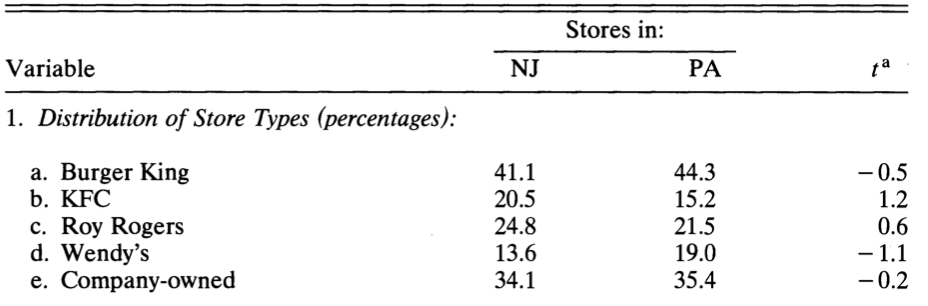
\includegraphics[width=2.25in]{./resources/ck_tab2b.png}\\
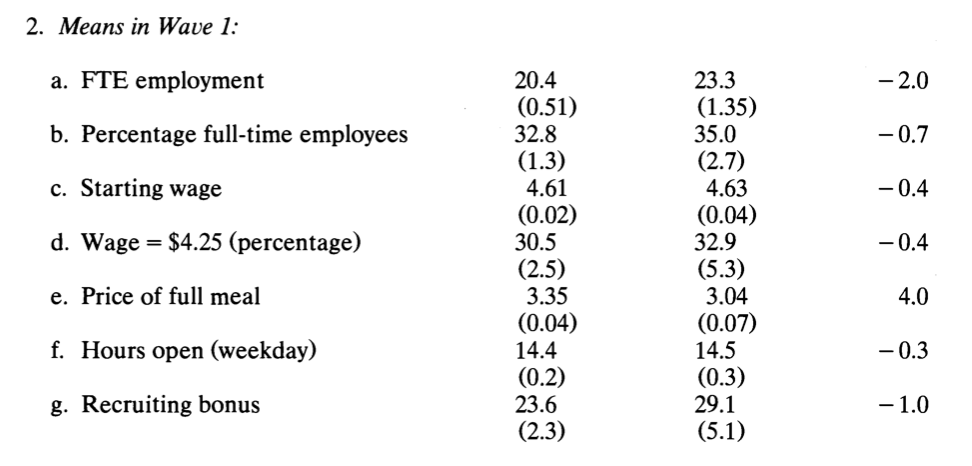
\includegraphics[width=2.25in]{./resources/ck_tab2c.png}\\
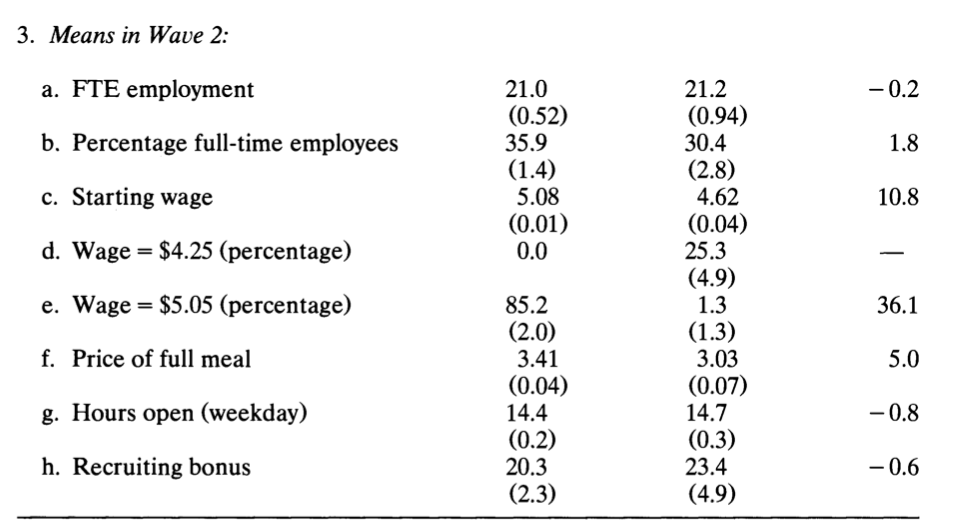
\includegraphics[width=2.25in]{./resources/ck_tab2a.png}
\end{center}
\end{frame}



\begin{frame}{Distribution of Wages}
\begin{center}
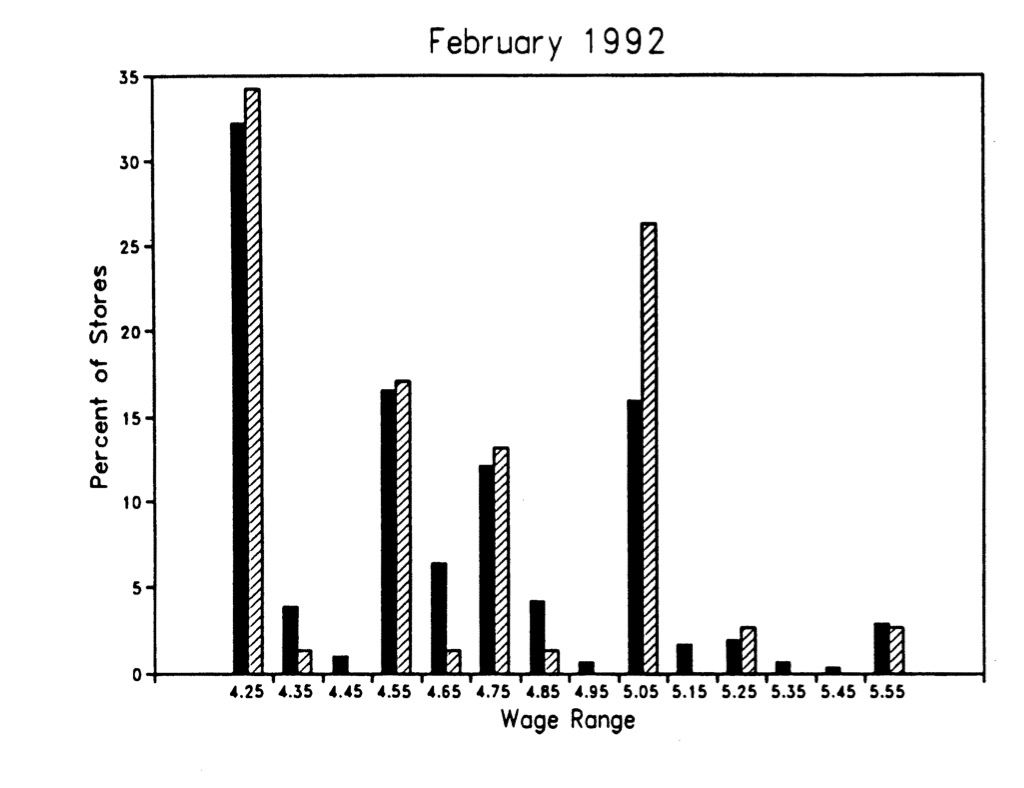
\includegraphics[width=2.75in]{./resources/ck_fig1b.png}
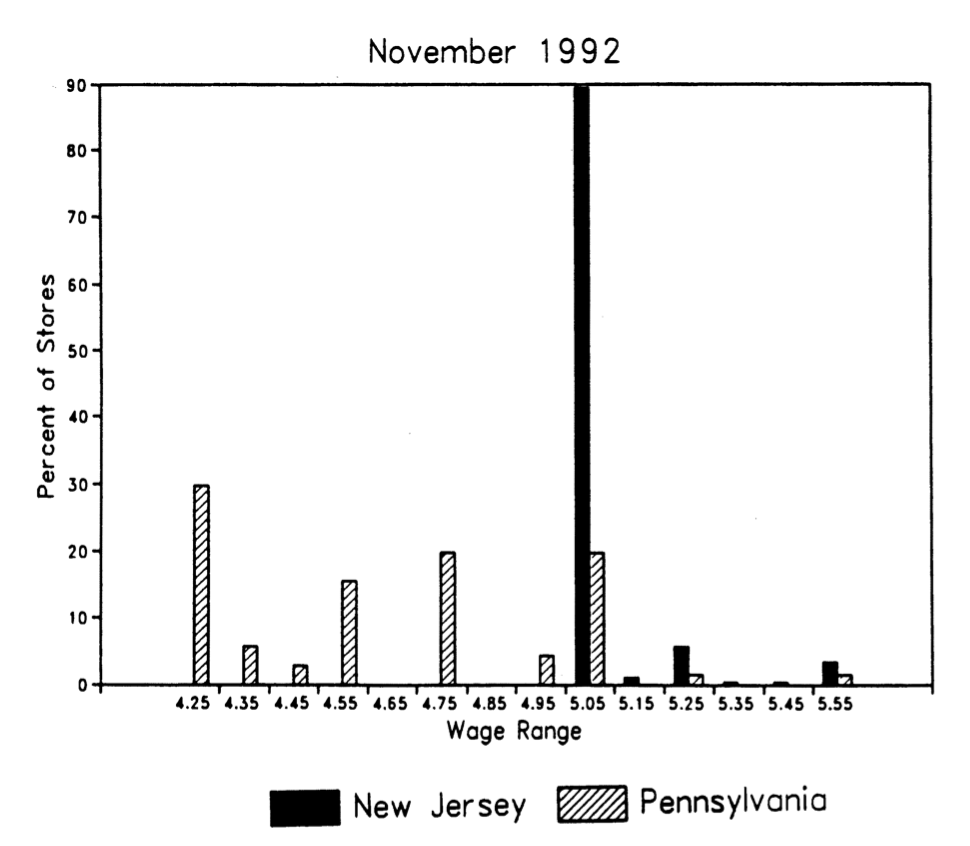
\includegraphics[width=2.5in]{./resources/ck_fig1a.png}
\end{center}
\end{frame}


\begin{frame}{Differences in Wages : 2 x 2 Table}
\begin{center}
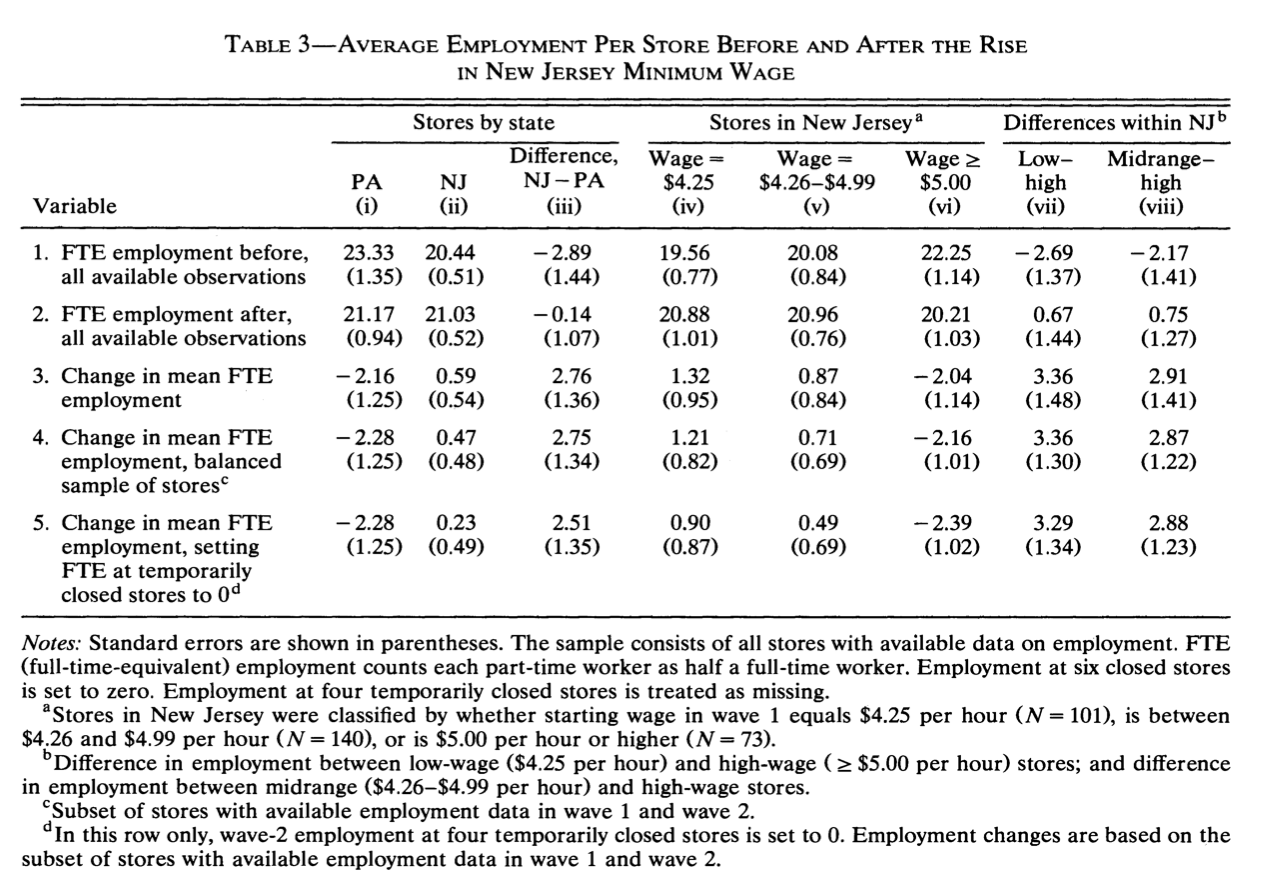
\includegraphics[width=4.25in]{./resources/ck_tab3.png}
\end{center}
\end{frame}

\begin{frame}{Outcome Equation}
\begin{itemize}
\item Differences lack any covariates (different fast food chains).
\item Also $\Delta_{PA}<0$ and $\Delta_{NJ} > 0$ (!)
\item Recall $i$ denotes stores, $t \in {1,2}$. Run the following regression:
\begin{align*}
Y_{it}&=\beta X_{it} +\alpha \cdot [i \in \text{NJ}] +  \gamma \cdot \text{After}_{t}  + \delta \cdot NJ_i \times After_{t} +u_{i}\\
Y_{it}&=\beta X_{it} +\alpha \cdot [\text{wage gap}_{i}] +  \gamma \cdot \text{After}_{t}  + \delta \cdot \text{wage gap}_{i} \times After_{t} +u_{i}
\end{align*}
\item $\alpha$ is mean difference between $NJ$ and $PA$
\item $\gamma$ is mean difference between period $1$ and $2$
\item $\delta$ is the parameter of interest, the \alert{difference in difference}
\item $\text{wage gap}_{i} = [\text{min wage}_{i,2}-w_{i1} ]_{+} =\max\{0, \text{min wage}_{i,2}-w_{i1}\} $.\\
 (How much do you need to raise $t=1$ wages to achieve minimum wage in $t=2$?)
\end{itemize}
\end{frame}

\begin{frame}{Differences in Wages}
\begin{center}
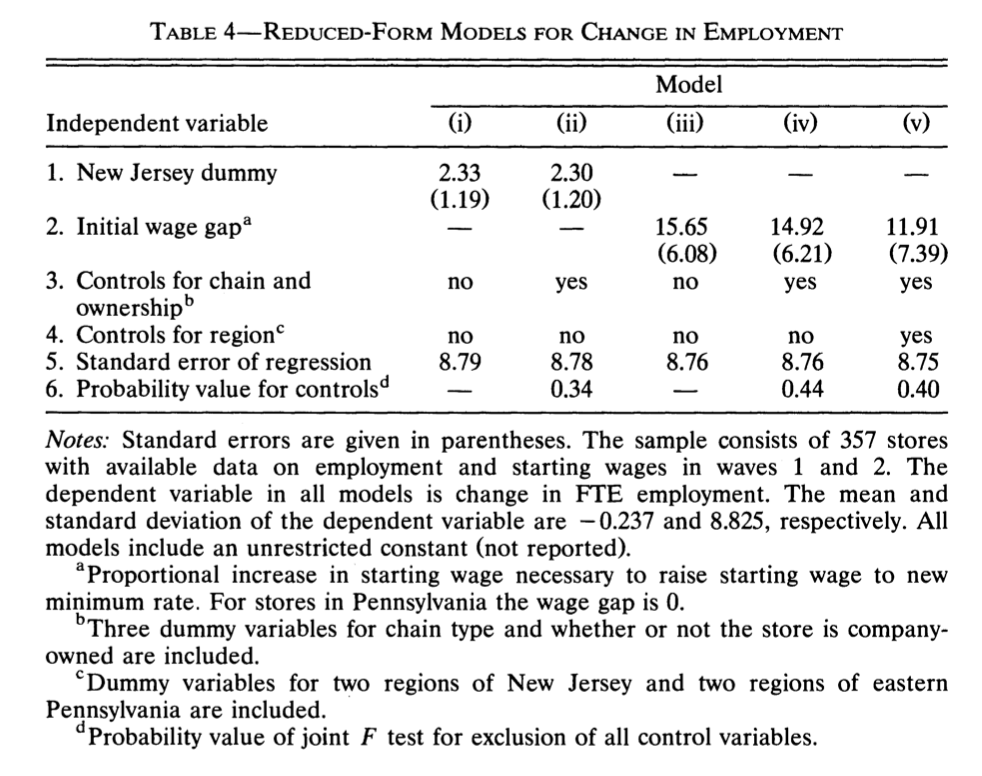
\includegraphics[width=4in]{./resources/ck_tab4.png}
\end{center}
\end{frame}


\begin{frame}{Parallel Trends}
\begin{figure}
\centering
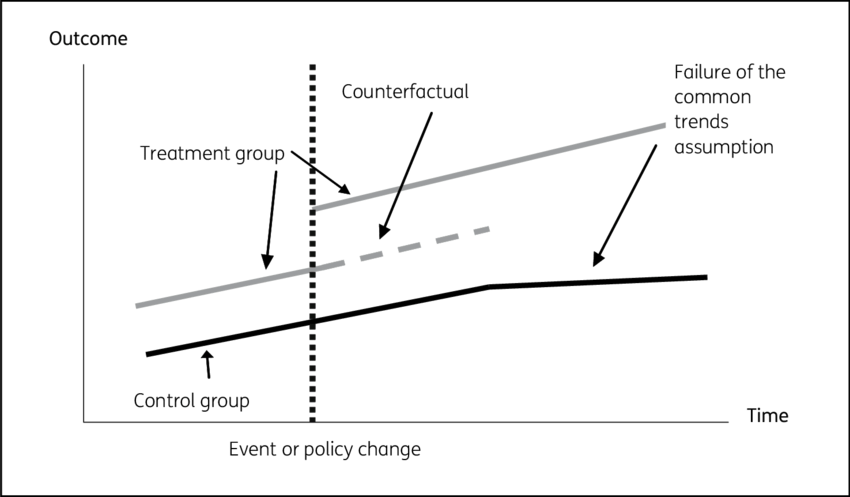
\includegraphics[width=5in]{./resources/common_trend.png}
\end{figure}
\end{frame}



\begin{frame}{Difference in Differences: Limitations}
\begin{enumerate}
\item Functional form restrictions
\begin{itemize}
\item \alert{Parallel trends} assumes that absent treatment that we add $\gamma_2 - \gamma_1$ to each unit
\item Because this is \alert{additive} it is not invariant to transformations $f(Y_{it})$ (ie: taking logs)
\end{itemize}
\item Parallel Trend Assumption is \alert{not testable}
\begin{itemize}
\item Best we can hope is that it looks similar in the pre-period
\end{itemize}
\item Compositional Effects: the treatment may affect who is in each group
\begin{itemize}
\item Restaurants could close in NJ and open nearby in PA to avoid minimum wage.
\item A good job training program may lead to migration, etc.
\item One approach: redefine the population so that it doesn't endogenously respond to treatment
\begin{itemize}
\item Recover something, but probably not ATT anymore...
\end{itemize}

\end{itemize}

\end{enumerate}

\end{frame}

\begin{frame}{Checking Pre-Trend: Card Krueger (2000)}
\begin{figure}
\centering
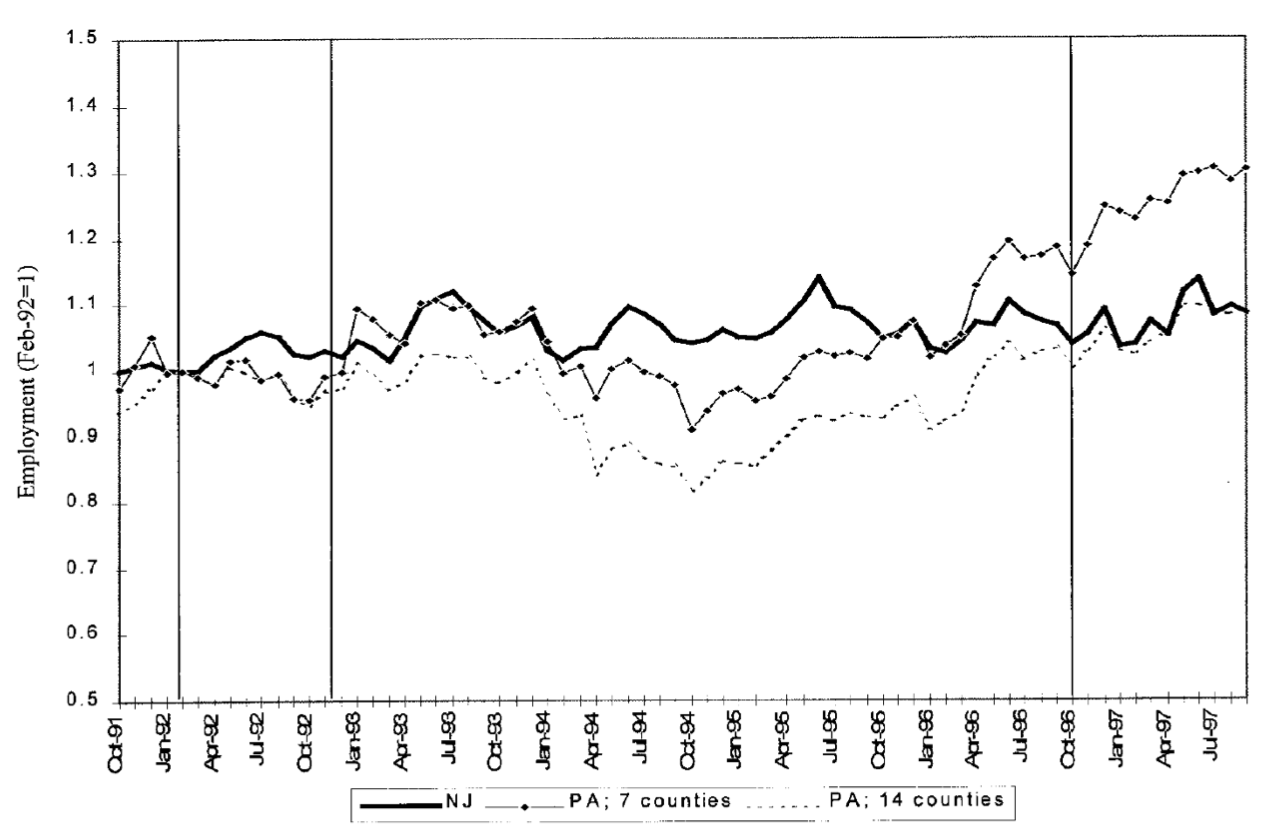
\includegraphics[width=4.5in]{./resources/card_krueger_2000.png}
\end{figure}
\end{frame}

\begin{frame}{The ``Ashenfelter Dip'' (Heckman and Smith 2000)}
\begin{figure}
\centering
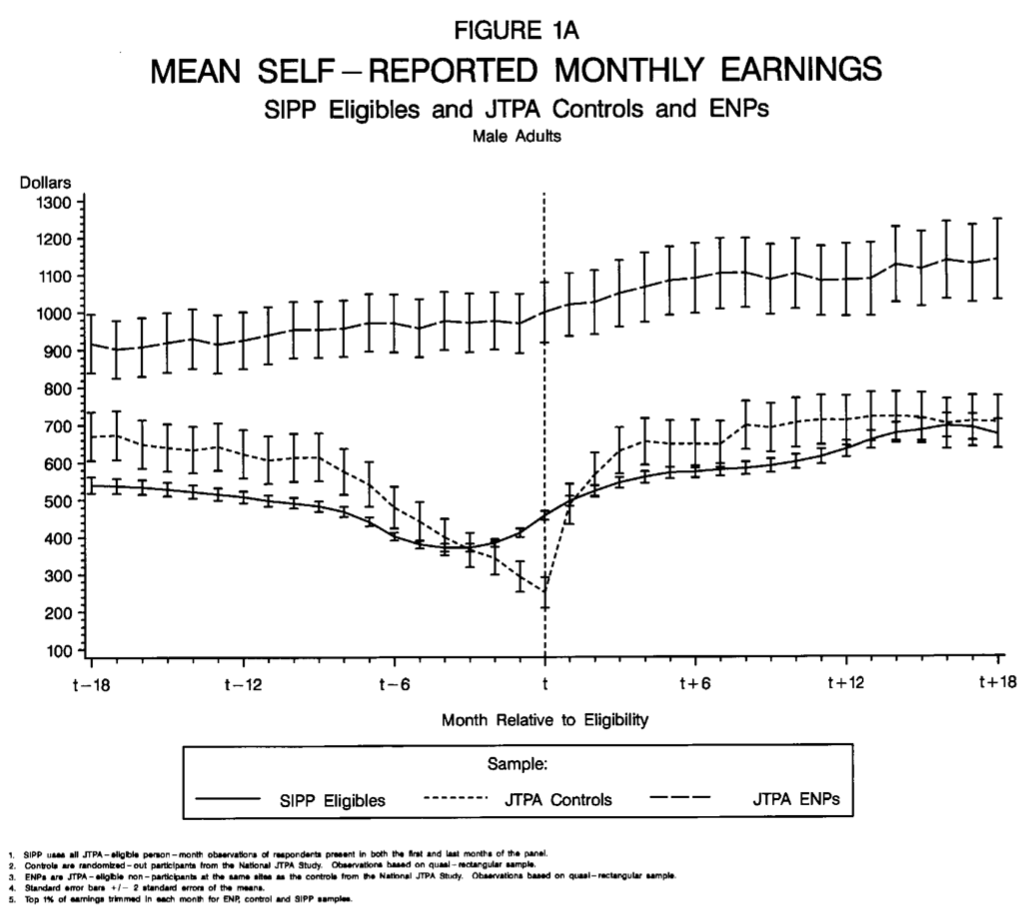
\includegraphics[width=4.25in]{./resources/ashenfelter_dip.png}
\end{figure}
\end{frame}



\end{document}

